\scanpage{84}
\margin{83}
\[
\begin{aligned}
n-\deleted{\unsure{\gamma}}-\deleted{(\unsure{\nu}-1)}-(\nu'-1)+\deleted{\unsure{\gamma}}\\
{}=n-(\nu'-1)\\
2n-\underbrace{[(\nu-1)+(\nu'-1)]}
\end{aligned}
\]
\figure{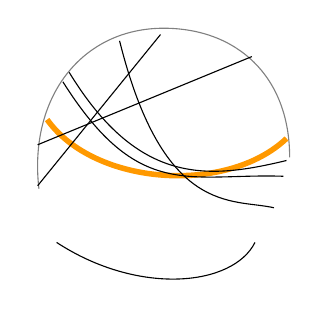
\begin{tikzpicture}[x=.8cm,y=.8cm]
\draw[gray] (.12,1.65)..controls(-.05,3.1)and(.8,4.2)..(2.1,4.2)..controls(3.25,4.2)and(4.1,3.45)..(4.1,2.15);
\draw[orange!80!yellow,line width=2pt] (.25,2.75) .. controls (1,1.7) and (3.1,1.55) .. (4.05,2.45);
\draw (.1,1.7)--(2.05,4.1);
\draw (.1,2.35)--(3.5,3.75);
\draw (.5,3.35) .. controls (1.7,1.45) and (2.5,1.9) .. (4,1.85);
\draw (.6,3.5) .. controls (1.7,1.7) and (2.8,1.8) .. (4.05,2.1);
\draw (1.4,4) .. controls (2.1,1.2) and (3.2,1.5) .. (3.85,1.35);
\draw (.4,.8) .. controls (1.7,-.05) and (3.2,.1) .. (3.55,.8);
\end{tikzpicture}}
\figure{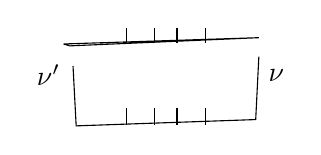
\begin{tikzpicture}[x=.8cm,y=.8cm]
\draw (0,1.3)--(3.1,1.4)--(.1,1.27)--(0,1.3);
\draw (.15,.95)--(.2,0)--(3.05,.1)--(3.1,1.1);
\foreach \x in {1,1.45,1.8,2.25}{\draw (\x,1.32)--(\x,1.55);\draw (\x,.02)--(\x,.28);}
\node[left] at (.1,.8) {$\nu'$};
\node[right] at (3.1,.8) {$\nu$};
\end{tikzpicture}}
\figure{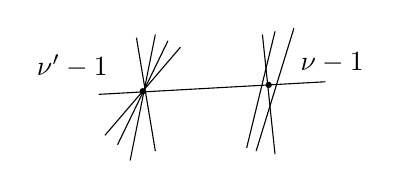
\begin{tikzpicture}[x=.8cm,y=.8cm]
\draw (0,1)--(3.6,1.2);
\fill (.7,1.05) circle (.05);\fill (2.7,1.15) circle (.05);
\draw (.6,1.9)--(.9,.1);\draw (.9,1.95)--(.5,-.05);\draw (1.1,1.85)--(.3,.2);\draw (1.3,1.75)--(.1,.35);
\draw (2.6,1.95)--(2.8,.05);\draw (2.8,2)--(2.35,.15);\draw (3.1,2.05)--(2.5,.1);
\node[left] at (.3,1.45) {$\nu'-1$};\node[right] at (3.05,1.5) {$\nu-1$};
\end{tikzpicture}}
